\section{Experiment}\label{secexp}
In this section, we demonstrate the experiments on the proposed interpretation.
In the first place,  we show the mechanism is reliable and generally agrees with global 
feature importance. Then we compare our interpretations to those of random 
forest and find it accord with the global feature importance better. Finally, 
we study the interpretations of real cases in our scenario and get a satisfied
analysis for them.

\subsection{Experiment setup}
The GBDT version in our experiment is the Scalable Multiple 
Additive Regression Tree(SMART)\cite{zhou2017psmart}, which is a distributed algorithm under the parameter server. 
Hundreds of billions of samples with thousands of features could be trained by the algorithm.
Not only the storage usage but also the running time cost is optimized 
without the loss of the accuracy.  

The training data is drawn from 
transactions under the scene of Fast Pay(FP)
in Alipay\footnote{https://global.alipay.com/}. A transaction is marked as a positive if it is reported as a fraud by the customer.
To keep a balanced ratio between positive and negative cases, only 1\% of normal transactions  are retained
 by random sampling. 

% 
%is an XML-based predictive model interchange format.
%PMML restricts a standard expression of different models and allows analysts share model among 
%different prediction implementations.  PMML include the process of data pre-processing and 
%post-processing along with model prediction. The structure of PMML files follows the order to 
%predict an instance, the compulsory parts of tree models are:
%\begin{enumerate}
%\item Header: general information about PMML document.
%\item Data Dictionary: field definitions in model.
%\item Model: contains the definition of the data mining model.
%\item Mining Schema: a list of all fields used in the model.
%\item Output: name all the desired output fields expected from the model.
%\end{enumerate}
\begin{figure}[th]
 \centering
 \includegraphics[width=0.65\textwidth]{pic/pmml.png}
    \caption{GBDT Model in PMML Format }\label{figpmml}
\end{figure}
\KZ{I suggest changing the background of this figure to white.}
Fig \ref{figpmml} is a fraction of GBDT model in Predictive Model Markup Language (PMML) format\footnote{http://dmg.org/pmml/v4-3/GeneralStructure.html}
and the tree embedded in it can be
 translate as shown in Fig \ref{figgbdt}. 
The element $Node$  is an encapsulation for a 
 tree node, which contains a predicative rule to choose itself or its siblings. The attribute $id$ 
 assigns a unique number to each node in a tree. The value of $score$ in a $Node$ is the 
 predicted value for an instance falling into it. $SimplePredicate$ is a simple boolean expression 
 indicating the split information. Our pre-trained model is stored as a PMML file. 
 JPMML\footnote{https://github.com/jpmml/jpmml-evaluator} is employed as the evaluator and
 we implement the proposed interpretation based on it.
 
\subsection{Consistency check}
We implement the feature contribution as the previous description in \cite{friedman2001greedy}. In order to make the interpretation
be independent of the training process of GBDT, the training algorithm is not changed in our experiment.
In order to get the distribution of instances in equation \ref{avgmod}, we use JPMML to predict
the training instances and record instance distributions on every node.  According to the tree structure in model and
instance distributions, the pre-process is done by back propagating the local increments  as shown in 
section \ref{secmech}. With the local increments, the feature contributions of the new instances could be computed. 
After interpreting lots of instances, we can get a distribution of feature contributions among the instances. 
The median is a robust estimator for the expectation of the general feature contribution and should somehow keep accordance with
the global feature importances metrics\cite{palczewska2013interpreting}.
\begin{figure}[htbp]
 \centering
 \includegraphics[width=0.8\textwidth]{pic/gbdtimp.png}
    \caption{Feature Importance and Feature Contribution Medians}\label{figimp}
\end{figure}

Fig \ref{figimp} plots the global Feature Importance(FI) for GBDT and Feature Contribution(FC) medians for every feature.
As we can see, this two statistics have similar distributions and are in good agreement. It proves that the
interpretation for GBDT is practical and reasonable.

\subsection{Comparison to Random Forest}
Following the experiment of last section,  we get a ranking of the feature contribution median. This ranking
is a measure of feature importance and reflects the quality of local interpretation.  We implement the work for
random forest in \cite{palczewska2013interpreting} and compare it with our ranking. For justice, we replace
the GBDT Feature Importance with Information Value(IV) as the importance metric. IV is a concept from 
information theory and shows the predictive strength for the features\cite{kullback1997information}. 
\begin{figure}[htbp]
 \centering
 \includegraphics[width=0.8\textwidth]{pic/ivimp.png}
    \caption{Interpretation: GBDT  v.s RF}\label{figiv}
\end{figure}

In Fig \ref{figiv}, we compute the intersection size on different variable coverage (i.e. Top 10-50 features
of IV).  $RF$ implies the method explained in section \ref{secrf}. $GBDT$ is the simple average strategy with
only the information in PMML file. $GBDTV2$ is the revised version in equation \ref{avgmod}. From the result,
our interpretations capture the importance better and the revised version works best.

\subsection{Case Study}
Besides the general evaluation, we analysis the 300 specific instances in the test data. Fig \ref{figcase} shows a case,
we only list some representative fields and divide them into 4 parts. The variables are ranked by IV (general feature
importance). Domain experts check the feature risk manually and draw the following conclusions:

\begin{itemize}
\item Part \uppercase\expandafter{\romannumeral1}: 
Variables in this section are with high IV, our interpretation is able to capture the features that are 
judged to be high risk(marked as blue fields). The feature with high IV but low risk (judging from
the feature value) is assigned a lower score, so the interpretation is good for instance-level contributions.
\item Part \uppercase\expandafter{\romannumeral2}:
 There are 2 variables(colored pink)  with high IV and marked high risk is missed by the interpretation, which 
 mainly due to its low occurrence in split features. The global importance of these two variables is also low and
 model interpretations are limit by the model quality.
\item Part \uppercase\expandafter{\romannumeral3}: 
Variables with median or low IVs are not caught by mistake and is assigned a low feature contribution for that case.
\item Part \uppercase\expandafter{\romannumeral4}: 
Several variables are considered to be high risk for the particular instance, even the general IVs of them are low. 
Our interpretation finds them out, which shows the superiority of the local feature contribution over the global feature importance.
\end{itemize}
\begin{figure}[htbp]
 \centering
 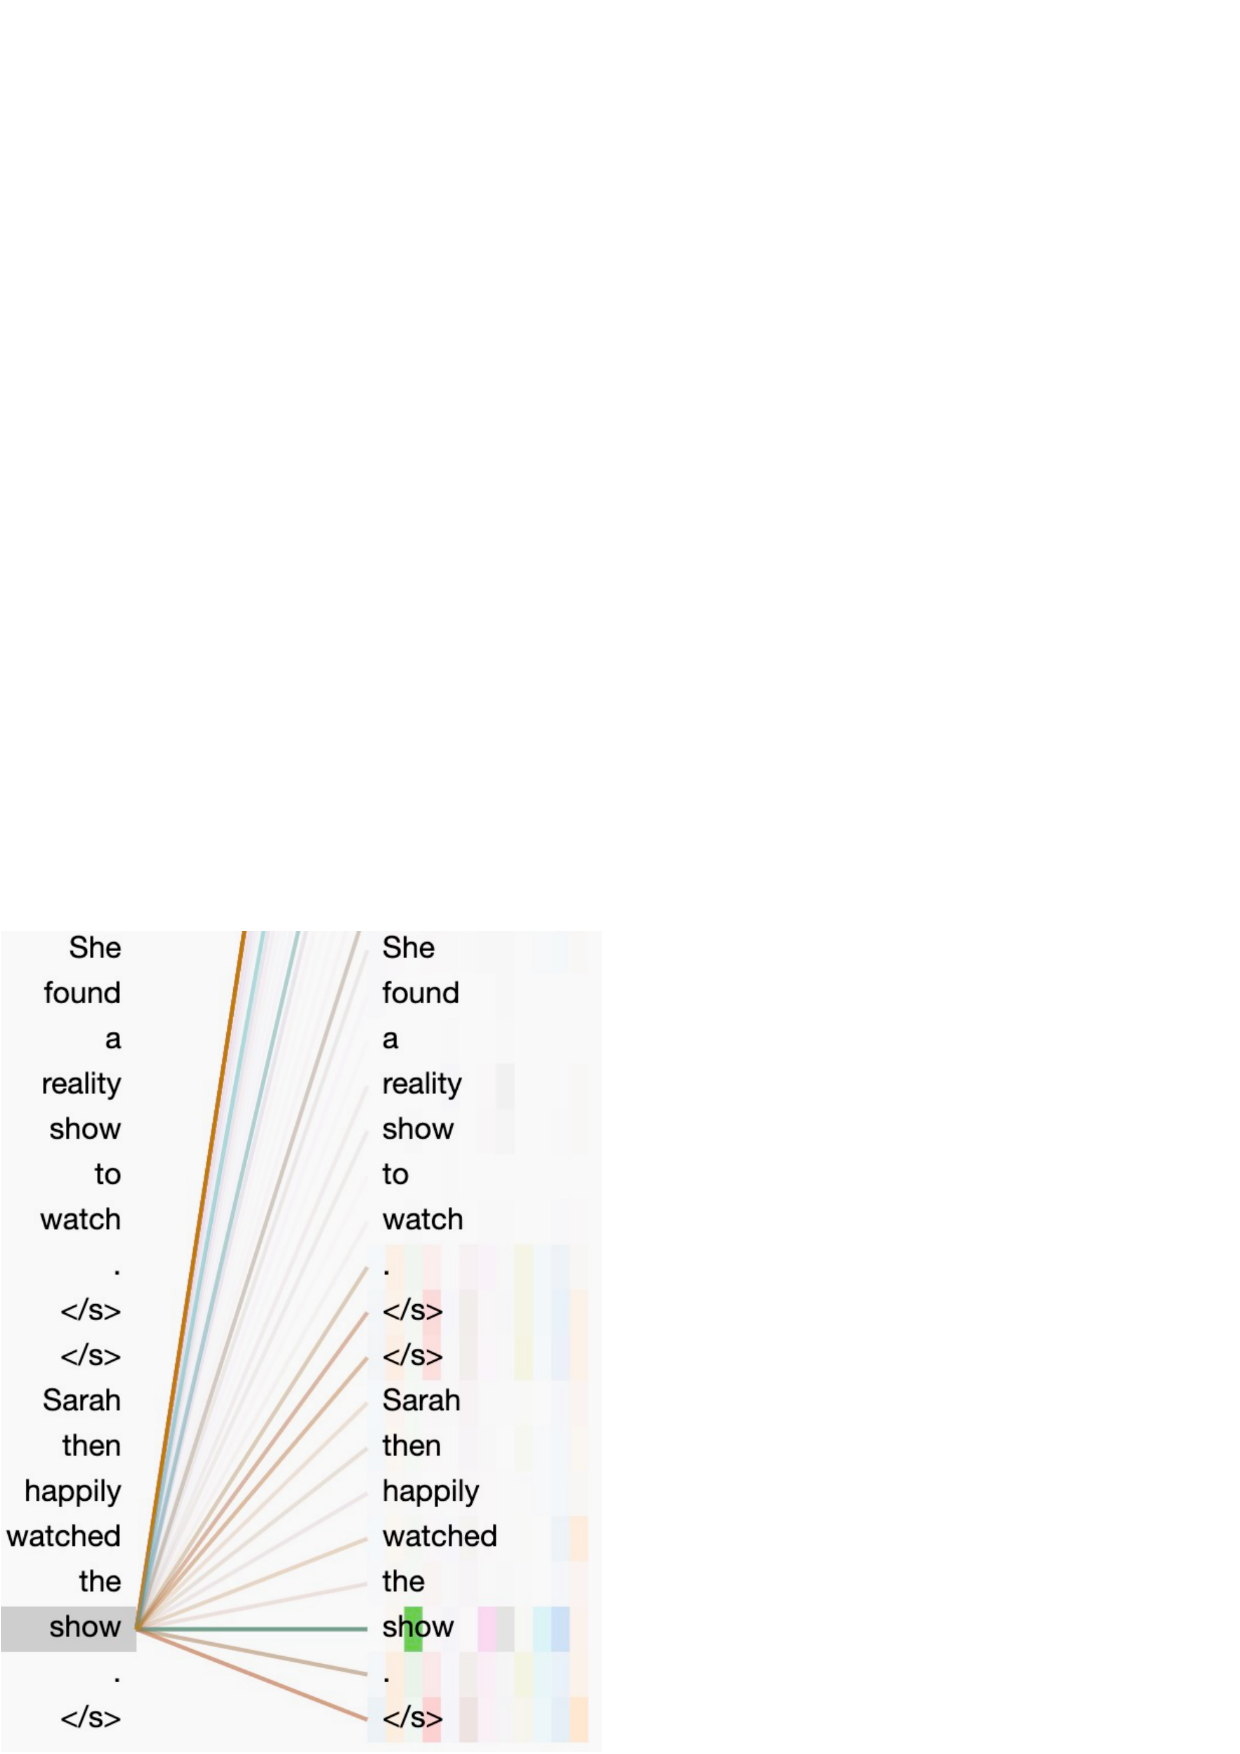
\includegraphics[width=0.9\textwidth]{pic/case.png}
    \caption{Case Study for Interpretation}\label{figcase}
\end{figure}
Further more, if we conduct interpretations on a batch of  fraud cases which are missed by the model,
the local feature contributions will help analysts improve the model.

